\documentclass[12pt, a4paper]{report}
\usepackage[outputdir=tmp]{minted}
\usepackage{graphicx}
\usepackage[export]{adjustbox}


\newenvironment{loggentry}[2]% date, heading
{\noindent\textbf{#2}\newline\{\marginnote{#1}\}\newline\\}{\vspace{1.0cm}}

\begin{document}
	\begin{titlepage}
		\centering
		
\includegraphics[width=0.15\textwidth]{res/inf.png}\par\vspace{1cm}
		{\scshape\LARGE UFRGS - Instituto de Informatica \par}
		\vspace{1cm}
		{\scshape\Large Volunteer Project\par}
		\vspace{1.5cm}
		{\huge\bfseries Kelvinlets Video Deformation\par}
		\vspace{2cm}
		{\Large\itshape Guilherme Gomes Haetinger\par}
		\vfill
		supervised by\par
		Dr. Eduardo S. L. \textsc{Gastal}

		\vfill

	% Bottom of the page
		{\large \today\par}
	\end{titlepage}

	\begin{figure}
		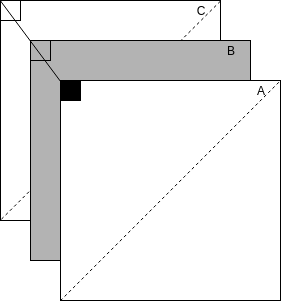
\includegraphics[scale=0.5, center]{./res/interpolationExample.png}
		\caption{3D Interpolation with Prism projection. (A) is the first grid involving the frame (B), and (C) is the second one.}
		\label{fig:newInterp}
	\end{figure}

	\begin{loggentry}{28-05-2019}{New Idea for 3D Interpolation}
		Based on the idea of interpolating 3D Cuboids on video frames, I wonder:
		are there other (better) ideas for this instead of Interpolating the tetrahedrons inside the prisms?
		One hypothesis is a prism projection on the video frames [fig.\ref{fig:newInterp}].	

		The idea of establishing Scan Conversion on the Frame mesh based solely on line interpolation between the preprocessed grids seems really faster than the tetrahedron approach.
		Whereas we would process every point inside a bounding box delimited by the corners of every tetrahedron inside a Cuboid (6 volumes), we now process one pixel related to 2 others, which colors will interpolate, and scan convert the remaining pixels of the frame with the produced ones, as we would do in the KelvinletsImageGL code.
		I like to call this new method 2 step interpolation.  
	\end{loggentry}

	\begin{loggentry}{30-05-2019}{Elaborating Implementation for 2 step Interpolation}
			Having in mind the Professor's advice to use a \textit{bin sort} alike algorithm, the main goal is to set which lines collide with each of the frames.
			We do that by assigning each vertex from the frame having 2 points: one in each deformed frame.
			Based on that, we can establish the color and position of the vertices.
			Now, considering the order that the vertices must be processed, we should run them by the time axis, i.e. Interpolate the same pixel position for each frame before moving to another position.    
	\end{loggentry}

	\begin{loggentry}{(01 - 03)-06-2019}{Project Structure}
		Creating the projects structure is a challenge.
		Separating a OpenGL application in modules is somewhat difficult because of the fact that many functions depend on predeclared variables, which means I need many arguments for a specific function.
		Therefore, I will, firstly, separate the needed functionalities in main components.
		These components are:
		\begin{itemize}
			\item Main
												
				This module will only serve to process the user arguments set in \textit{argv} and to call the other methods with these arguments.
			
			\item VideoDeformator
										
				This module will be in charge of processing the arguments given by the \textit{Main} modules in order to execute the Kelvinlets \textit{grab} function in each vertex.
				It will produce a new set of vertex arrays for the ones in the video input (regularized vertices).
				This module will include the \textbf{glm} and the \textbf{glfw3} library, since it will depend on the data structures involving linear algebra as well as the ones defined for OpenGL visualization.

				\begin{itemize}
					\item[$\ast$] InterpolationFrame

						This data structure should hold every line in charge of interpolating each vertex of the frame.
					
					\item[$\ast$] Line

						This data structure should hold the information to interpolate a line in a given point in the time axis.

					\item[$\ast$] Deformation

						Abstraction of a deformation vector(initial position, final position and brush size).

					\item[$\ast$] KelvinletsTransformer

						Class that provides the execution of the Kelvinlets equation.
				
				\end{itemize}
			
			\item VideoVisualizer

				This module will be responsible for the video rendering, i.e. the communication of the program with the deformed  video data and the graphic card.
				To do this, we must use the OpenGL library, for which we will need the vertices positions and colors, as well as the order in which they will be accounted for the triangle mesh rendering in the \textbf{TRIANGLE\_STRIP} method.
				We are supposed to import, for these reasons, \textbf{glfw3} and \textbf{glew} for the data structures and graphic card communication functions.

		\end{itemize}

		For the sake of the project and organization, I also developed a \textbf{logger} for the application.
		This will make debugging much cleaner and easier.
		All I have to do to get specific output (errors, fatal errors, warnings and general debugging logs) is call the program in the following way:
	
	\begin{minted}{shell}

env KELVIN="FATAL"|"ERROR"|"WARNING"|"CORRECT"|"DEBUG" ./kelvin
	
	\end{minted}
	\end{loggentry}

	\begin{loggentry}{(04 - 05)-06-2019}{Implementing The Project}
		Started with the simpler structures(Deformation, Point and Line).
		These classes should be working properly, so I will probably test them in the main function before implementing the others, which require more work.
		\begin{itemize}
				\item Deformation

					Simple getters and setters.
				
				\item Point

					Simple getters.			
				
				\item Line

					This one took a little more time than it should.
					The main functionality for this class was the interpolation of values (color and position).
					What confused me was the approach that should bee used for this purpose.
					Firstly, I thought I should use the line between the two points to elaborate its equation and use it to find the \textit{xy} coordinates for the point that had the Z-axis correspondent to the frame index.
					That approach was mode complicated, since the 3D line equation is a little bit harder to find and to understand.
					The best approach ended up being the simple use of a linear interpolation value, as the following equation shows:

					$$Z = t * Za + (1 - t) * Zb$$
					$$X = t * Xa + (1 - t) * Xb$$
					$$Y = t * Ya + (1 - t) * Yb$$
					
					Considering that we already know the value of Z, we can replace its value and find out the following: $t =  (Z - Za)/(Zb - Za)$, which is the reason between the distances.
		\end{itemize}
	
		I ended up having to add more modules for the sake of organization and clean code. These are:

		\begin{itemize}
				\item VideoGL

					This module is in charge of receiving the input video, setting up its frame's vertex array, color array and index array, initializing the rendering process and calling the RenderableFrames draw method to display the video.
					It will probably turn the VideoVisualizer obsolete (incorporated more than it was supposed to).

				\item VideoWindow

					The idea behind this component is to initialize and instantiate every variable RenderableFrames and VideoGL will need to render into the created window.

				\item Proportions

					This is not a module but a header.
					It was just a way I thought of keeping the \textit{width, height} and \textit{length} (the number of frames) altogether.
		\end{itemize}

	\end{loggentry}

	\begin{loggentry}{06-06-2019}{Implementing the Renderable Video Logic}		

		Firstly, I decided to create 2 constructors for \textbf{VideoGL}:
		One that receives a video path and, thus, will create its own arrays from the video source;
		and one that will receive a RenderableFrame array and Proportions, which will, than initialize every component needed.
		This will be needed when 1.reading a video source and 2.turning the InterpolationFrames into renderable.
		
		\begin{itemize}
				\item Initializing the Arrays

					\begin{itemize}
							\item[$\ast$] Vertex Array

								Initializing the vertex array is quite simple:
								We will need a 2-dimensional \textit{for}, a variable to keep track of the axis (\textit{xy}) and another to keep track of the array index.
								The result of this \textit{for} will be used as a template for each RenderableFrame.
								Each one of these will have, now, the value of its \textit{z} axis built in the class.
								The needed changes in the project will be necessary to view the video.
								The code goes like this:
	
							\begin{minted}{cpp}

int size = this->getWidth() * this->getHeight() * 2;
GLfloat * templateArray = (GLfloat *) malloc(size * sizeof(GLfloat));
int index = 0;
for(int y = 0; y < this->getHeight(); y++)
	for(int x = 0; x < this->getWidth(); x++){
		templateArray[index] = (GLfloat) normalize(x);
		templateArray[index + 1] = (GLfloat) normalize(y);
		index += 2;
	}

for(int frame = 0; frame < this->getLength(); frame++)
	renderableFrames[frame].setVertices(templateArray);

							\end{minted}

							Where \textit{normalize} takes a coordinate normal to the frame size domain and takes it into the OpenGL screen domain [-1; 1];

							\item[$\ast$] Color Array

								The basic differences between the creation of the vertex array and the color array is that we will need the video to take the color of its pixels, that there will be no template, since every array will be, probably, different and that the size of the array will be multiplied by 3 (\textit{RGB}) instead of 2 (\textit{xy}).
								To implement the first difference, we will need the Video function to get each color channel, solely.
								The second difference will be a bit harder, since we will, now, have to create a 3-dimensional \textit{for} and run through the video frames as we process the new arrays.
								We can do the second one by something like this:

								\begin{minted}{cpp}

VideoCapture video(videoPath);
...
int size = this->getWidth() * this->getHeight() * 3;
uint8_t * buff = (uint8_t *)malloc(size * sizeof(uint8_t));
Mat frame;
video >> frame;
memcpy(buff, mat.ptr(0), mat.cols*mat.rows * sizeof(uint8_t) * 3);
...
//Color for pixel in index
GLfloat R = ((GLfloat) buff[index + 2])/256;
GLfloat G = ((GLfloat) buff[index + 1])/256;
GLfloat B = ((GLfloat) buff[index])/256;
...
								\end{minted}

								In this case, \textit{index} is both the array's and frame's counter. They are both processed the same way.

							\item[$\ast$] Index Array

	\begin{figure}
		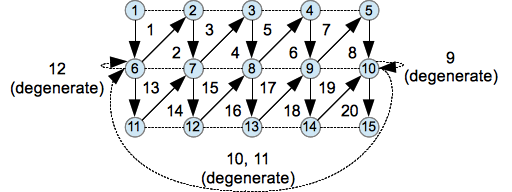
\includegraphics[scale=1.0, center]{./res/strip.png}
		\caption{Drawing a grid with Triangle Strips}
		\label{fig:newInterp}
	\end{figure}

								This array, however simple it is to maintain (is always the same or a given proportion), it is the hardest one to generate.
								Since we will be using the \textbf{GL\_TRIANGLE\_STRIP} method of mesh generation for its little memory usage given a regularized vertex grid, we will need to implement the Index array with its rules and restrictions.
								The best way to do so is to follow the rules as exemplified on fig.\ref{fig:newInterp}.
								In every line between the extremes, we should create undrawable triangles (e.g. [6, 6, 2], which has 2 of the same index, which is a line without thickness) so that we can join one side of the triangle with the other, creating a flow. Since there would not be any difference if we apply the redundancy on the extreme lines, we will do that for the sake of simplicity. 
								Processing this array will only happen once, since it is equal in each vertex. The creation function goes like this:

								\begin{minted}{cpp}

int size = getNumberOfIndices(this->getWidth(), this->getHeight());
GLuint * templateArray = (GLuint *) malloc(size * sizeof(GLuint));
int counter = 0;

for(int y = 0; y < this->getHeight(); y++){
	//adds redundancy for 1st element on row
	templateArray[counter] = y * this->getWidth();
	counter++;
	for(int x = 0; x < this->getWidth(); x++){
		//joins the vertex with its correspondent
		//column-wise on the row below
		int columnOutset = y * this->getWidth();
		int position = columnOutset + x;
		templateArray[counter] = position; 
		templateArray[counter+1] = position + this->getWidth();
		counter += 2;
	}
	//adds redundancy for the last element in the row below
	//(before heading to the beginning of the same row)
	templateArray[counter] = (y+2) * this->getWidth() - 1;
}

								\end{minted}
	
					\end{itemize}
		\end{itemize}
		
	\end{loggentry}
\end{document}
